% !TeX spellcheck = it_IT
\section{5G}

Con il 5G, vengono aggiunti \textit{sempre più casi d'uso diversi tra loro}, e quindi il relativo supporto. Ci sono diversi casi d'uso completamente differenti, come ad esempio:
\begin{itemize}
	\item Multi-hop communication: comunicazione a più salti tra dispositivi per estendere la copertura e migliorare la connettività, utile in ambienti urbani o in aree remote

	\item Device-to-device communication and cooperative devices: comunicazione diretta tra dispositivi senza passare dalla rete centrale, per aumentare efficienza e ridurre la latenza	

	\item Ultra-reliable communication: comunicazioni ad altissima affidabilità, ad esempio per infrastrutture critiche come reti elettriche o trasporti

	\item Massive machine communication: connessione simultanea di un gran numero di dispositivi IoT, tipico di fabbriche smart, logistica e sensori ambientali	

	\item Inter-vehicular/vehicular-to-road communication: comunicazioni tra veicoli e tra veicoli e infrastrutture stradali per supportare la guida autonoma e la sicurezza stradale

	\item Ultra-dense deployments: aree con altissima densità di dispositivi connessi, come uffici o stadi, dove il 5G garantisce prestazioni elevate nonostante l'affollamento.
\end{itemize}

Si ampia il range di frequenze: va da $300MHz$ a $300GHz$. Comprende diverse fasce di frequenza.

\paragraph{Classificazione International Telecommunication Unit ITU:} Secondo l'ITU le applicazioni possono essere classificate in tre principali categorie di utilizzo:
\begin{itemize}
	\item \textbf{Enhanced Mobile Broadband (eMBB)}
	\begin{itemize}
		\item Servizi orientati alle persone

		\item Elevata banda

		\item HD Streaming, AR/VR
	\end{itemize}

	\item \textbf{Ultra-reliable and Low-latency communication (uRLLC)}
	\begin{itemize}
		\item Servizi orientate alle industrie

		\item Bassissima latenza e affidabilità

		\item Controllo remoto, guida autonoma
	\end{itemize}

	\item \textbf{Massive Machine Type Communications (mMTC)}
	\begin{itemize}
		\item alta densità di connessioni (anche con bassa quantità di dati trasmessi)

		\item smart cities/smart agriculture
	\end{itemize}
\end{itemize}

\begin{center}
	\resizebox{\linewidth}{!}{\renewcommand{\arraystretch}{1.2}
		\begin{tabular}{l | l}
			\textbf{Key Performance Indicator KPI} & \textbf{Minimum Performance Requirement} \\
			\hline
			\multirow{2}{*}{Peak Data Rate} & Downlink: 20 Gbps \\
			\cline{2-2}
			& Uplink: 10 Gbps \\
			
			\hline 
			\multirow{2}{*}{Peak Spectral Efficiency} & Downlink: 30 bps/Hz \\
			\cline{2-2}
			& Uplink: 15 bps/Hz \\
			\hline
			
			\multirow{2}{*}{User-Experienced Rate} & Downlink: 100 Mbps \\
			\cline{2-2}
			& Uplink: 50 Mbps \\
			\hline
			
			5th-Percentile User & Downlink: 0.12 bps/Hz $\approx$ 0.3 bps/Hz \\
			\cline{2-2}
			Spectral Efficiency & Uplink: 0.045 bps/Hz $\approx$ 0.21 bps/Hz \\
			\hline
			
			\multirow{2}{*}{Average Spectral Efficiency} & Downlink: 3.3 bps/Hz $\approx$ 9 bps/Hz \\
			\cline{2-2}
			& Uplink: 1.6 bps/Hz $\approx$ 6.75 bps/Hz \\
			\hline
			
			Area Traffic Capacity & 10 Mbps/m$^2$ (Indoor Hotspot) \\
			\hline
			
			\multirow{2}{*}{User Plane Latency} & 4ms - eMBB \\
			\cline{2-2}
			& 1ms - URLLC \\
			\hline
			
			Control Plane Latency & 20ms \\
			\hline
			
			Connection Density & 1'000'000 devices per km$^2$ \\
			\hline
			
			\multirow{3}{*}{Energy Efficiency} & The support for two aspects: \\
			\cline{2-2}
			& (1) Efficient data transmission in a loaded case \\
			\cline{2-2} 
			& (2) Low energy consumption when there are no data \\
			\hline
			
			Reliability & $1-10^{-5}$ ($99.999\%$) \\
			\hline
			
			Mobility & Up to 500km/h \\
			\hline
			
			Mobility Interruption Time & 0ms \\
			\hline
			
			\multirow{2}{*}{Maximal Bandwidth} & 100 MHz for sub-6 GHz \\
			\cline{2-2}
			& 1 GHz for mmWave \\
			\hline
	\end{tabular}}
\end{center}

Le "direzioni" dell'evoluzione per 5G sono: 
\begin{itemize}
	\item Maggiore spettro
	\item Maggiore efficienza spettrale
	\item Riuso spaziale
	\item "Softwarizzazione" della rete
\end{itemize}

%End L19

\subsection{Tecnologie abilitanti al 5G}

\subsubsection{Software Defined Networking SDN}

La struttura di un'applicazione di rete "normale" (senza SDN), consiste di un layer per control e data assieme, il quale si occupa sia del flusso di controllo che del flusso di dati. I dispositivi nella rete hanno al loro interno gli algoritmi di controllo e le regole di forward. 

SDN "toglie" dai dispositivi di rete la \textbf{parte di controllo}, la quale viene \textbf{centralizzata} in un SDN controller: questo è collegato con tutti i dispositivi e implementa le regole di controllo. 

Tutte le regole di controllo sono implementati ad un \textbf{livello software} al di sopra del data layer. Offre un'interfaccia unificata all'esterno della rete e permette una conoscenza topologica globale della rete stessa.

\begin{center}
	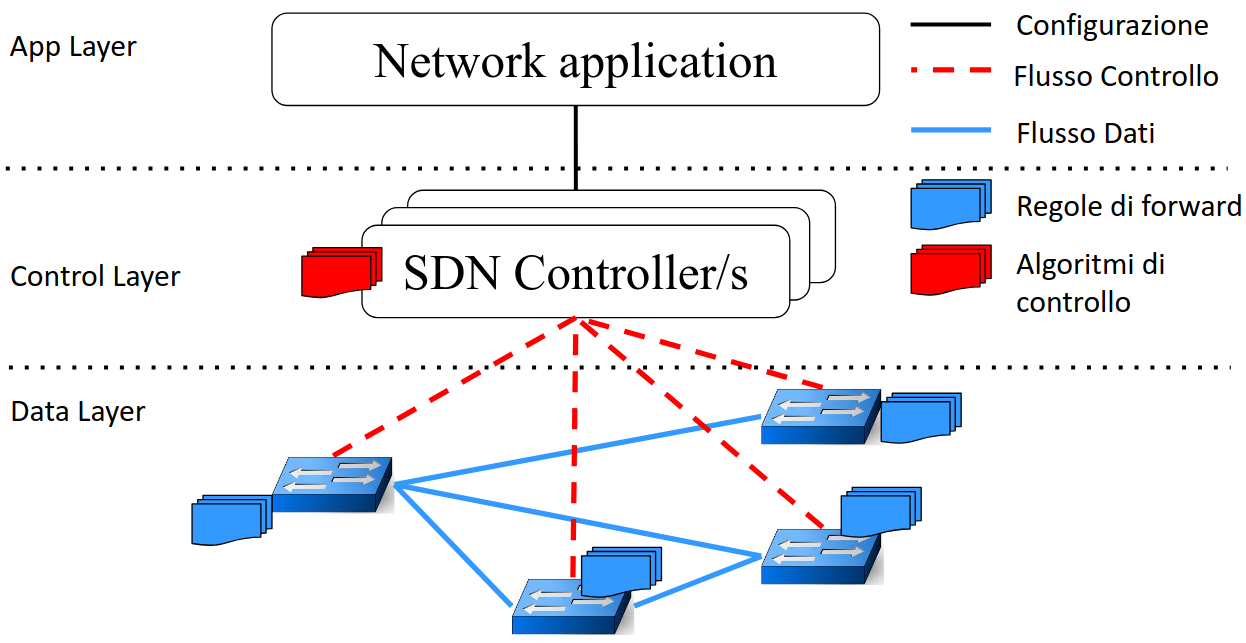
\includegraphics[width=0.8\linewidth]{img/5g/sdn1}
\end{center}

I dispositivi di rete usano un linguaggio in grado di comunicare con l'SDN controller; si ha un linguaggio apposito per la comunicazione tra controller e switch.

Si può lavorare anche in maniera reattiva: una volta ricevuto un pacchetto, il dispositivo richiede al controller la regola relativa. In questo modo il controller può inviare/gestire la regola anche per gli altri dispositivi presenti all'interno della rete.

Nel networking tradizionale, una volta definiti control e data plane non si possono più modificare i layer, con SDN e fixed-function data plane si possono modificare le funzionalità di controllo a livello software. 

L'evoluzione vuole andare verso SDN con data plane programmabile, si ha SDN in cui tutto è programmabile, ovvero anche il livello dati ha funzionalità programmabili.

\begin{center}
	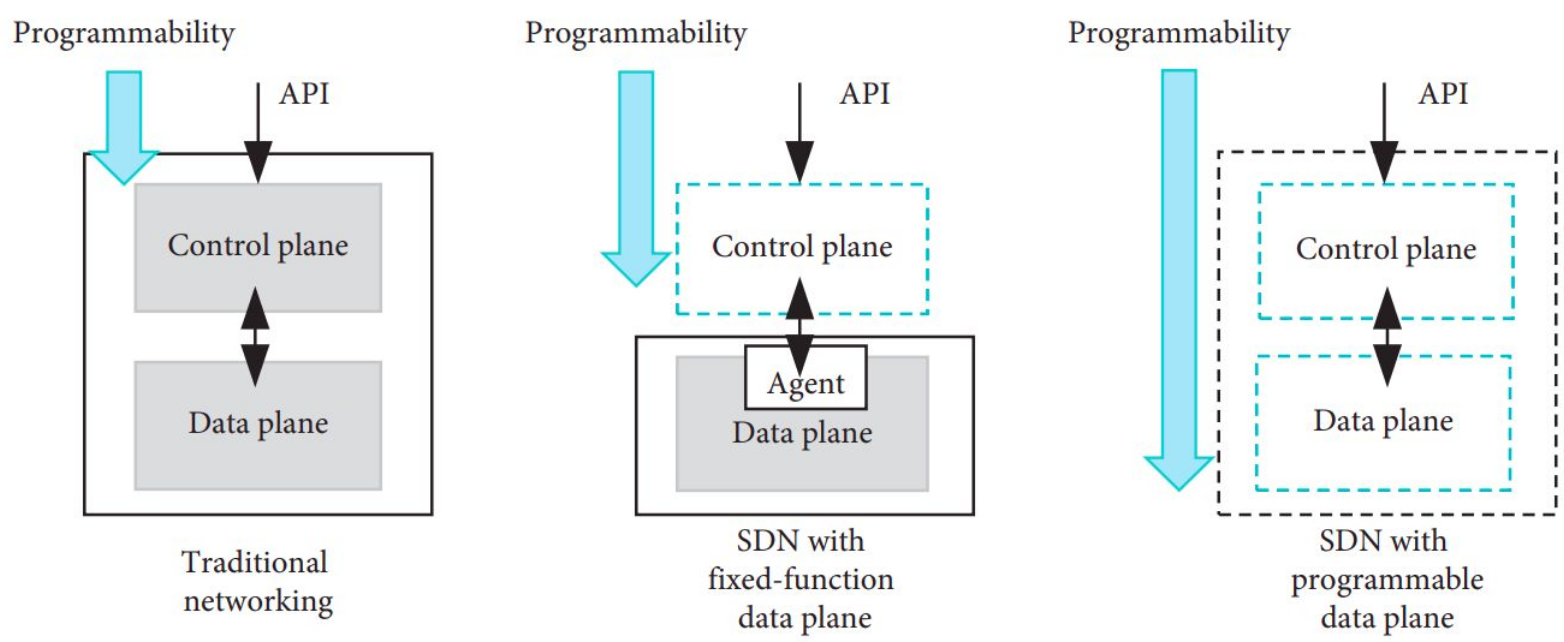
\includegraphics[width=0.95\linewidth]{img/5g/sdn2}
\end{center}

L'architettura prevede una parte di parsing programmabile: si può programmare come il pacchetto ricevuto viene processato. 

Se data plane è fisso, si possono programmare che regole utilizzare, ma queste devono essere implementate dal data plane, altrimenti nulla. Questo permette molta più flessibilità; le reti cambiano molto velocemente e questo permette di adattare i meccanismi alle condizioni della rete on-the-fly. Si vuole far arrivare il software fino al data link, al bordo del livello fisico.

I vantaggi sono diversi:
\begin{itemize}
	\item flessibilità nella gestione della rete

	\item visione centralizzata, quindi ottimizzazione del routing

	\item semplificazione della gestione a livello applicativo (OSS/BSS)

	\item testing e configurazione di nuovi protocolli di rete più semplice e veloce
\end{itemize}

Ma ci sono anche delle sfide: 
\begin{itemize}
	\item i controller diventano un single point of failure

	\item permette di reagire real-time: ma questo deve essere fatto in modo efficiente

	\item ottimizzazione del numero di regole: gestione ottimizzata delle tabelle di forwarding, gestione e garanzia dell'isolamento di reti di overlay (reti logiche), gestione della complessità

	\item sicurezza: controllare il controller vuol dire controllare la rete
\end{itemize}

\subsubsection{Network Function Virtualization NFV}

Prima dell'avvento di questa tecnologia, ogni componente necessitava hardware dedicato; si aveva una soluzione hardware specifica e la corrispondente soluzione software, strettamente legata.

Con NFV vengono separate le funzionalità hardware e software. A partire da un hardware "standard" si possono installare le implementazioni software delle funzionalità di rete richieste. Viene virtualizzata la parte software della funzionalità di rete per poi istanziarla a bordo di hardware standard. Questo permette di avere istanze in base a dove e quanto necessario. 

Ma come si implementano le funzionalità di rete che implementano il servizio? \textbf{Service Function Chain (SFC)}: grafo delle funzionalità necessarie, requisiti del servizio da creare.

Il \textbf{NFV Orchestrator} contiene dei template per determinate funzionalità e le istanzia secondo la configurazione necessaria, ovvero in base alla SFC. 

Si occupa anche di dove metterle (resource allocation); decide dove posizionare le istanze delle funzionalità necessarie sulle risorse hardware a disposizione, in modo che vengano rispettati tutti i vincoli: capacità dei nodi, passaggio, performance, \dots

\paragraph{Architettura NFV:} Standardizzato da \href{https://www.etsi.org/}{\texttt{ETSI}}. La base sono risorse hardware e, tramite virtualizzazione, vengono offerte risorse virtualizzate. Tutto questo diventa una \textbf{NFV Infrastructure}, ovvero l'infrastruttura su cui istanziare le risorse di rete virtualizzate.

Sulla base di questo vengono montate le \textbf{Virtual Network Functions}. Per ogni istanza viene tenuta traccia del suo stato di funzionamento: \textbf{Element Management System (EMS)}.

Il tutto si interfaccia alla rete operatore (BSS/OSS) tramite \textbf{NFV MANO} (Management and Orchestration). All'interno della NFV MANO si trovano
\begin{itemize}
	\item \textbf{Virtual Infrstructure Manager (VIM)}: definisce quali risorse sono disponibili e dove
    
	\item \textbf{VNF Manager (VNFM)}: gestisce le funzionalità di rete istanziate, presenti e future. Collegato al VIM per dire effettivamente \textit{cosa fare}, poi sarà lui che procederà all'istanziazione

	\item \textbf{Orchestrator}: coordina VNFM e VIM. Inoltre è collegato alla rete operatore per ricevere ed orchestrare le richieste all'interno della rete
\end{itemize}

I \textbf{descrittori} sono modelli per i contratti tra le varie componenti del NFV MANO, metadati strutturati che permettono all'orchestrator, VNFM e VIM di sapere cosa fare e come.

\begin{center}
	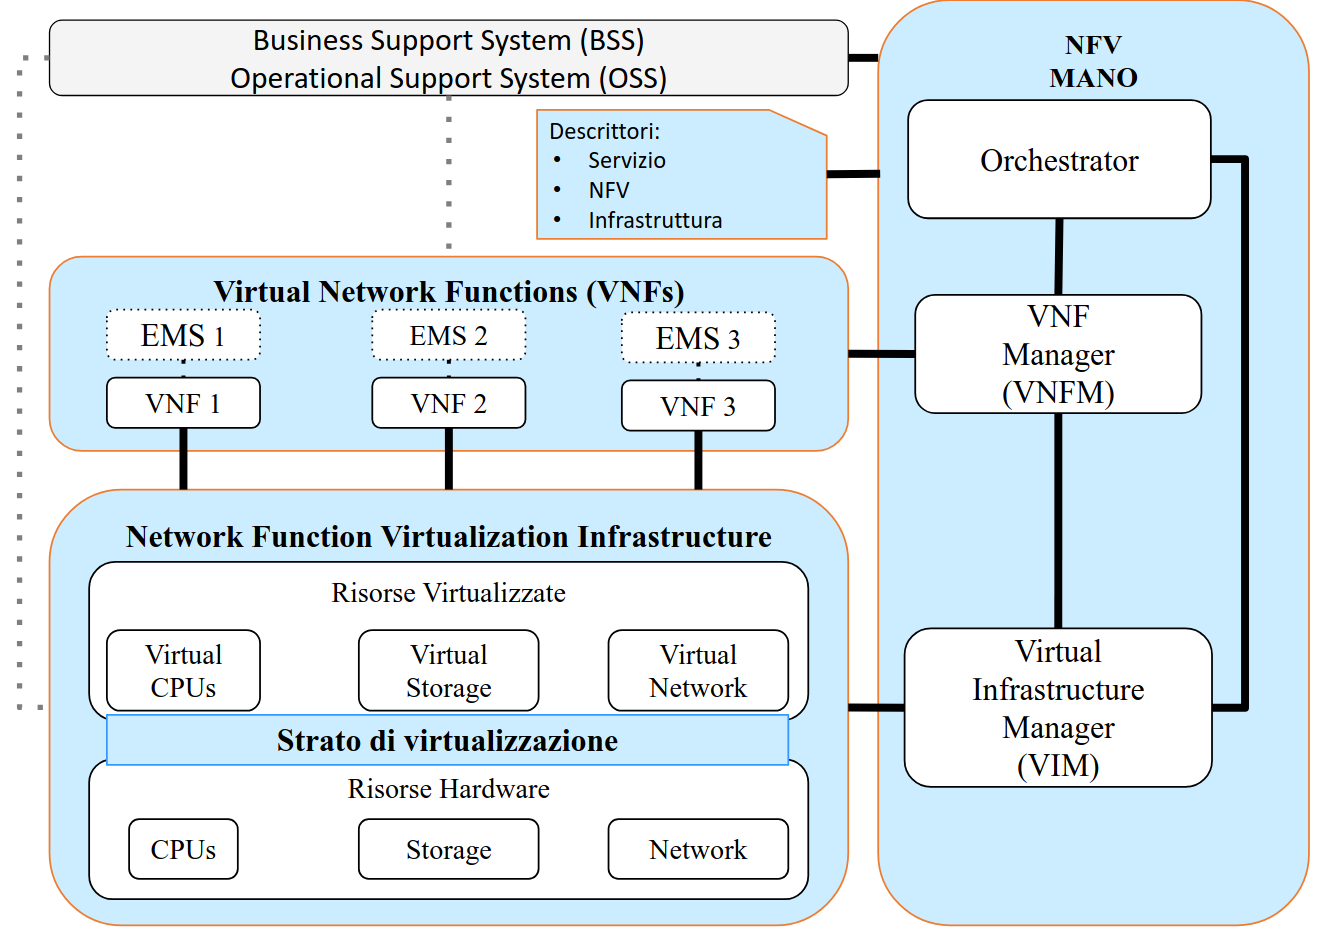
\includegraphics[width=0.95\linewidth]{img/5g/nfv1}
\end{center}

Vantaggi di NFV: 
\begin{itemize}
	\item flessibilità, scalabilità, agilità della rete e dei servizi; intrinseco nella virtualizzazione

	\item indipendenza hardware e software; si possono fare modifiche senza cambiare nient'altro, ad esempio: risolvere un bug senza cambiare l'hardware

	\item rapida prototipizzazione e introduzione di nuovi servizi, operatori e utenti finali

	\item uso delle risorse ottimizzato e condiviso
\end{itemize}

Sfide: 
\begin{itemize}
	\item le prestazioni devono essere comparabili con l'hardware dedicato, bisogna garantire certe prestazioni, nonostante l'overhead di virtualizzazione; le VFN vanno migliorate il più possibile, anche in termini di performance

	\item gestione efficiente delle risorse: servono tecniche ad hoc per ogni caso d'uso

	\item più software è presente, più problemi di sicurezza possibili esistono

	\item gestione della fase di transizione: devono coesistere hardware e software network function (non possiamo soppiantare la rete istantaneamente)

	\item gestione multi-tenant: più operatori di servizio possono condividere risorse hardware
\end{itemize}

\subsection*{Cloud + NFV + SDN}

Le prime due sezioni erano tecnologie abilitanti al 5G, il quale usa Cloud, SDN e NFV.

Partendo da un data center (molto) distribuito, si aggiungono le NFV sui vari componenti della rete ed i collegamenti tra questi vengono gestiti tramite SDN controller.

\subsection{Centralized-RAN C-RAN e Virtual-RAN V-RAN}

L'attuale architettura eNodeB è composta da Remote Radio Head RRH e Baseband Unit BBU, questo richiede: 
\begin{itemize}
	\item alimentazione
	
    \item condizionamento
	
    \item alto carico computazionale sulla BBU
	
    \item coordinamento via X2 per ridurre interferenze
	
    \item limitata visione dello stato degli altri eNodeB
	
    \item un singolo standard: solo 4G
\end{itemize}

Come si può densificare questa struttura? Per ogni antenna bisogna inserire tutte le componenti specificate: costoso e poco pratico. 

Per risolvere questo problema viene separata la RRH dai livelli superiori (MAC in su), ponendoli in remoto (ma non \textit{troppo remoto}, comunque c'è un vincolo geografico, 1km max circa). Vengono usate delle \textbf{Virtual Baseband Unit vBBU}, con sopra tutte le tecnologie necessarie, permettendo anche una migliore gestione in base al carico (virtualizzato).

Questo permette:
\begin{itemize}
	\item riduzione CAPEX (capital expenditure): si riduce il numero di apparati e si può riusare il sito, anche per introdurre nuove tecnologie RAT

	\item riduzione OPEX (operational expenditure): minor consumo energetico, ottimizzazione delle risorse BBU remote, gestione dinamica della potenza delle celle

	\item migliori prestazioni: migliore gestione delle interferenze, densificazione delle celle in maniera più sostenibile (dal punto di vista dell'operatore mobile)

	\item Multi-RAT, più tecnologie possono coesistere in una sola vBBU
\end{itemize}
\begin{center}
	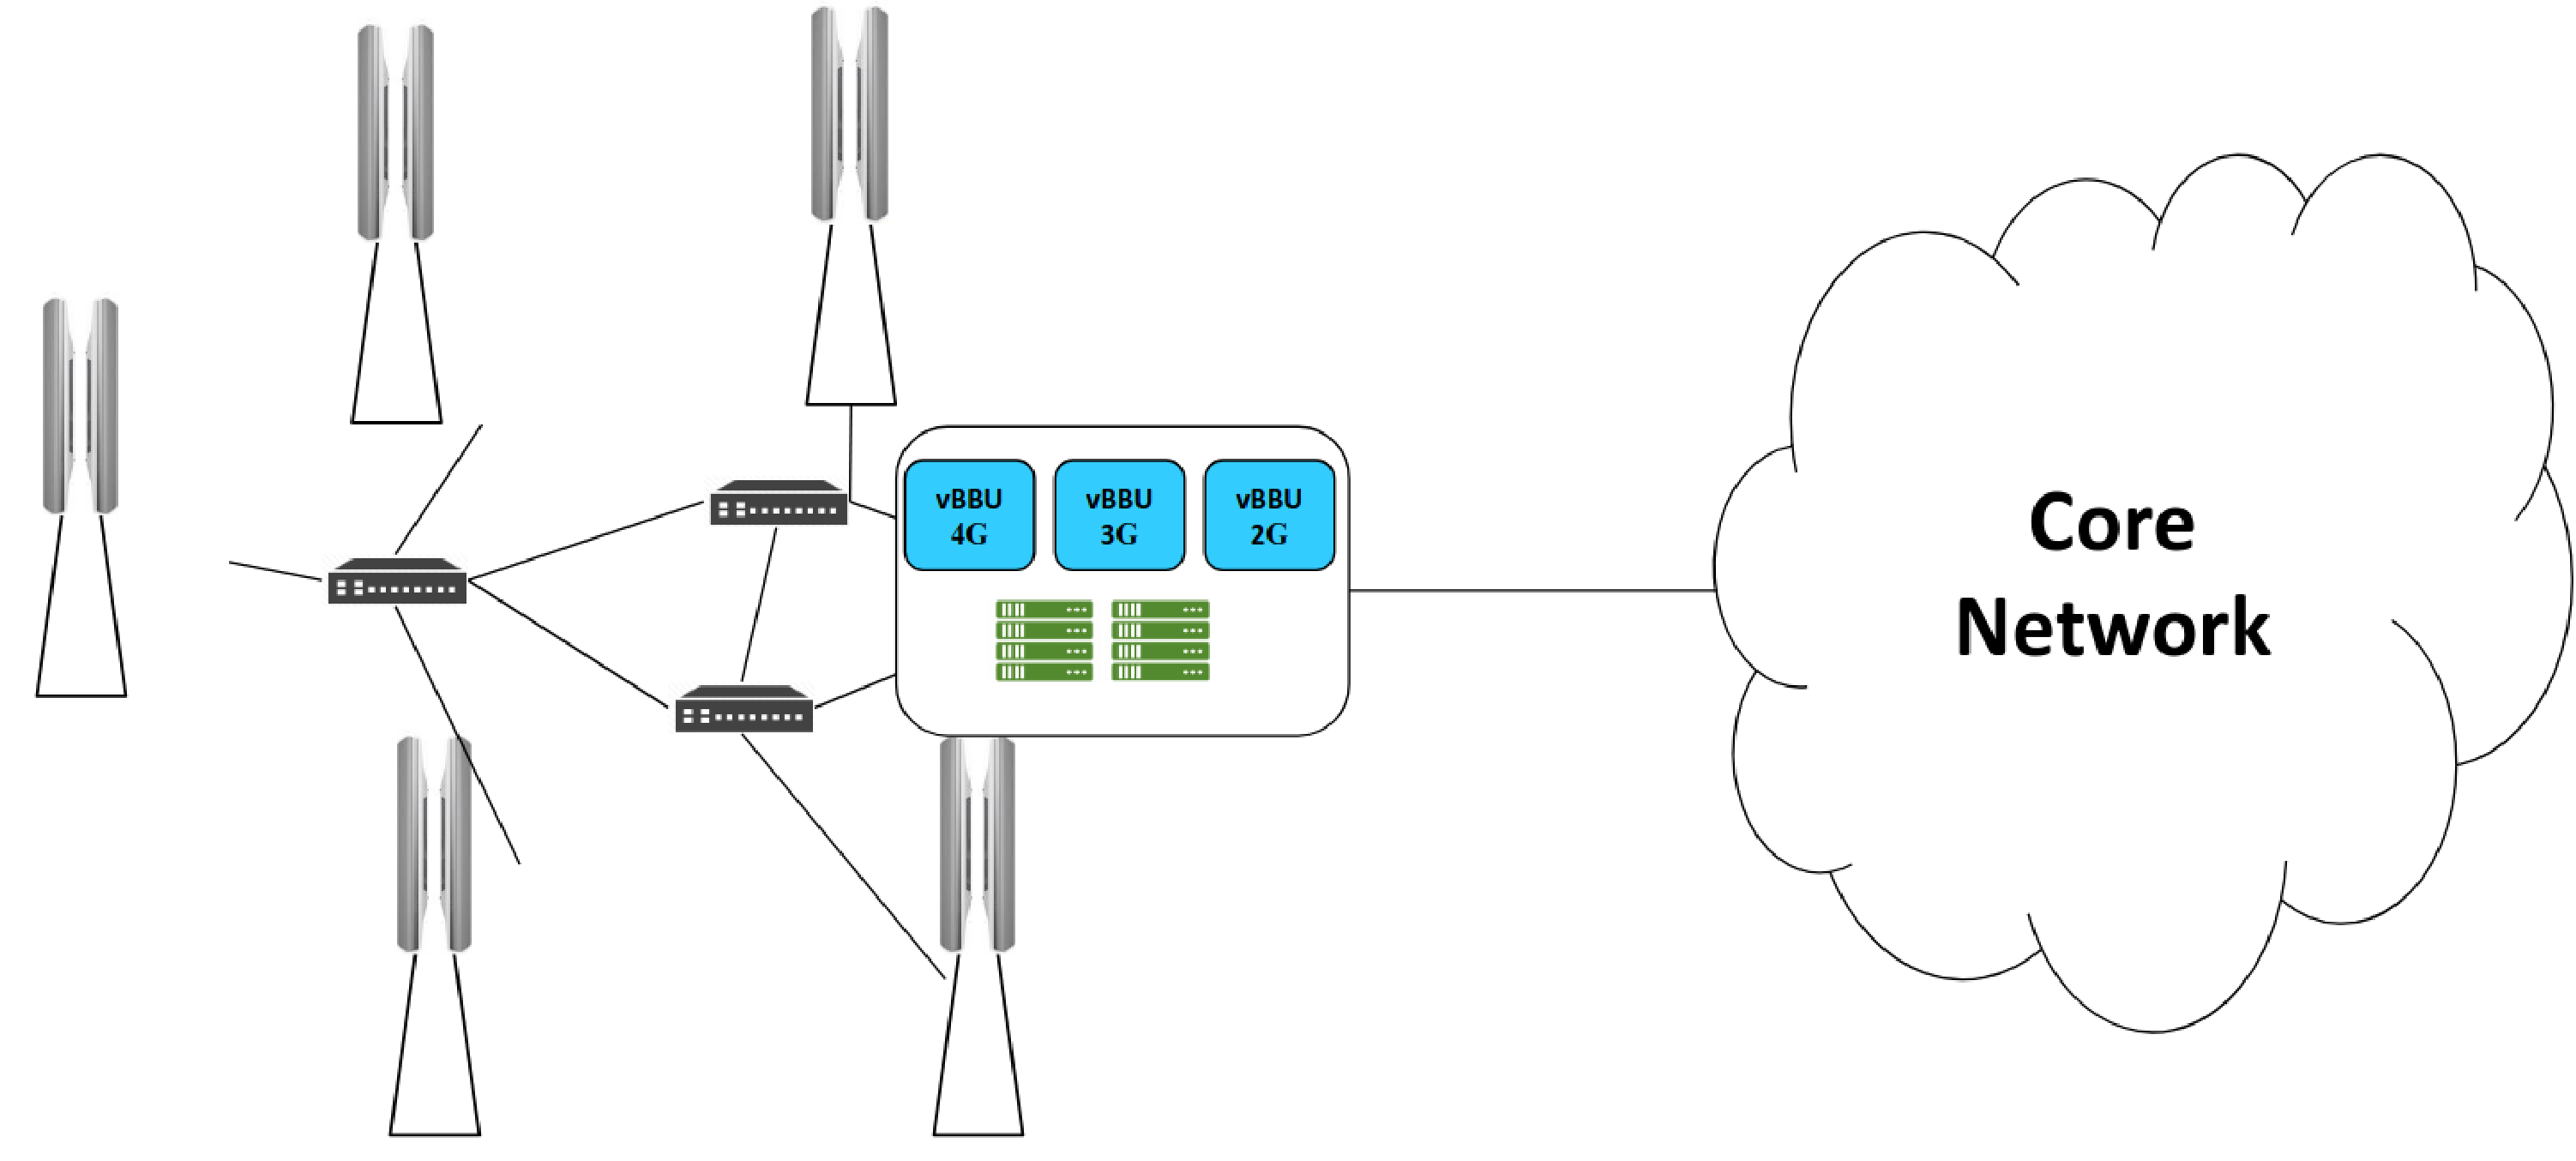
\includegraphics[width=0.98\linewidth]{img/5g/vbbu}
\end{center}

Per scalare la rete è sufficiente installare nuove RRH, senza dover aggiungere BBU, al posto della quale è necessario solo scalare orizzontalmente la vBBU già esistente (permetterne più istanze in parallelo, i.e., aumentare le performance). 

Tramite un singolo data center si possono gestire molte BS, risultando in una migliore gestione.

\subsection*{Cloud Computing}

Dai, sai come funziona, \href{https://it.wikipedia.org/wiki/Cloud_computing}{\texttt{ma nel caso}}. Una struttura tipica:
\begin{center}
	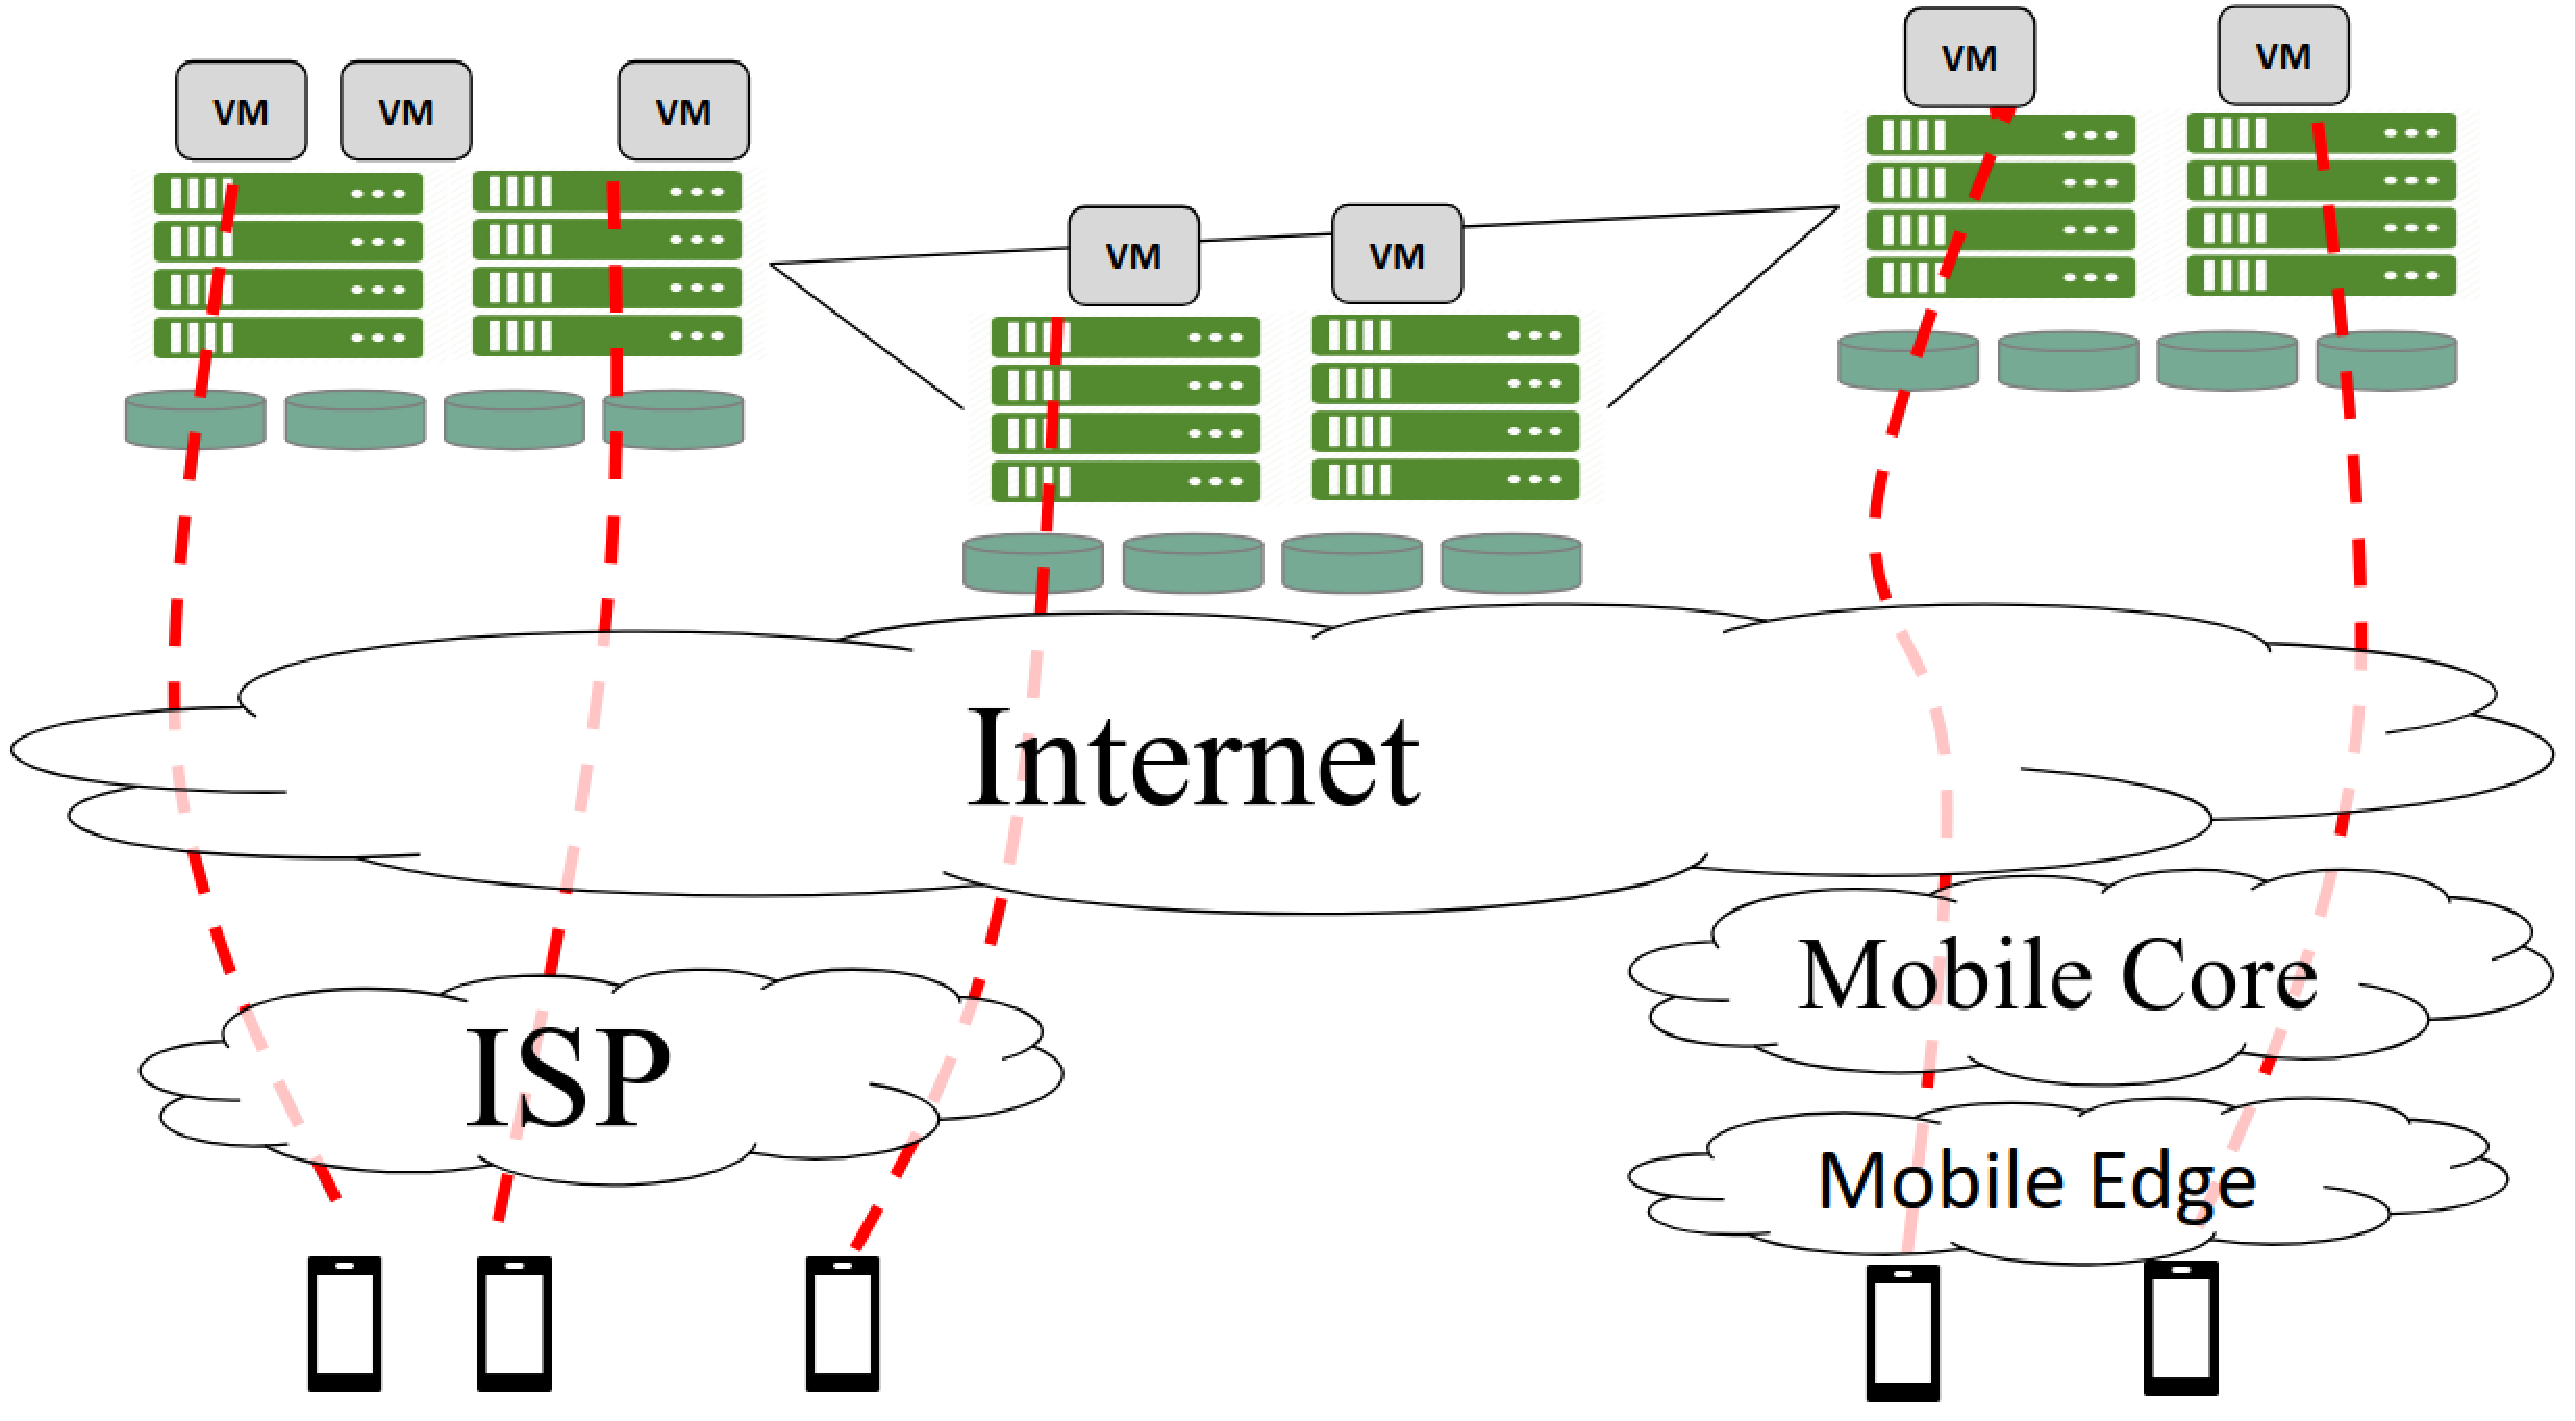
\includegraphics[width=0.8\linewidth]{img/5g/clud}
\end{center}

Questo potrebbe avere (relativamente) elevata latenza per i servizi, elevato jitter (deviazione standard sul delay alta), rendendo applicazioni near real-time difficili da realizzare.

\subsection{Mobile Edge Computing MEC (ETSI)}

Mobile Edge Computing (chiamato anche Multi-access Edge Computing). Si vuole avere delle risorse computazionali il più vicino possibile all'utente. 
\begin{center}
	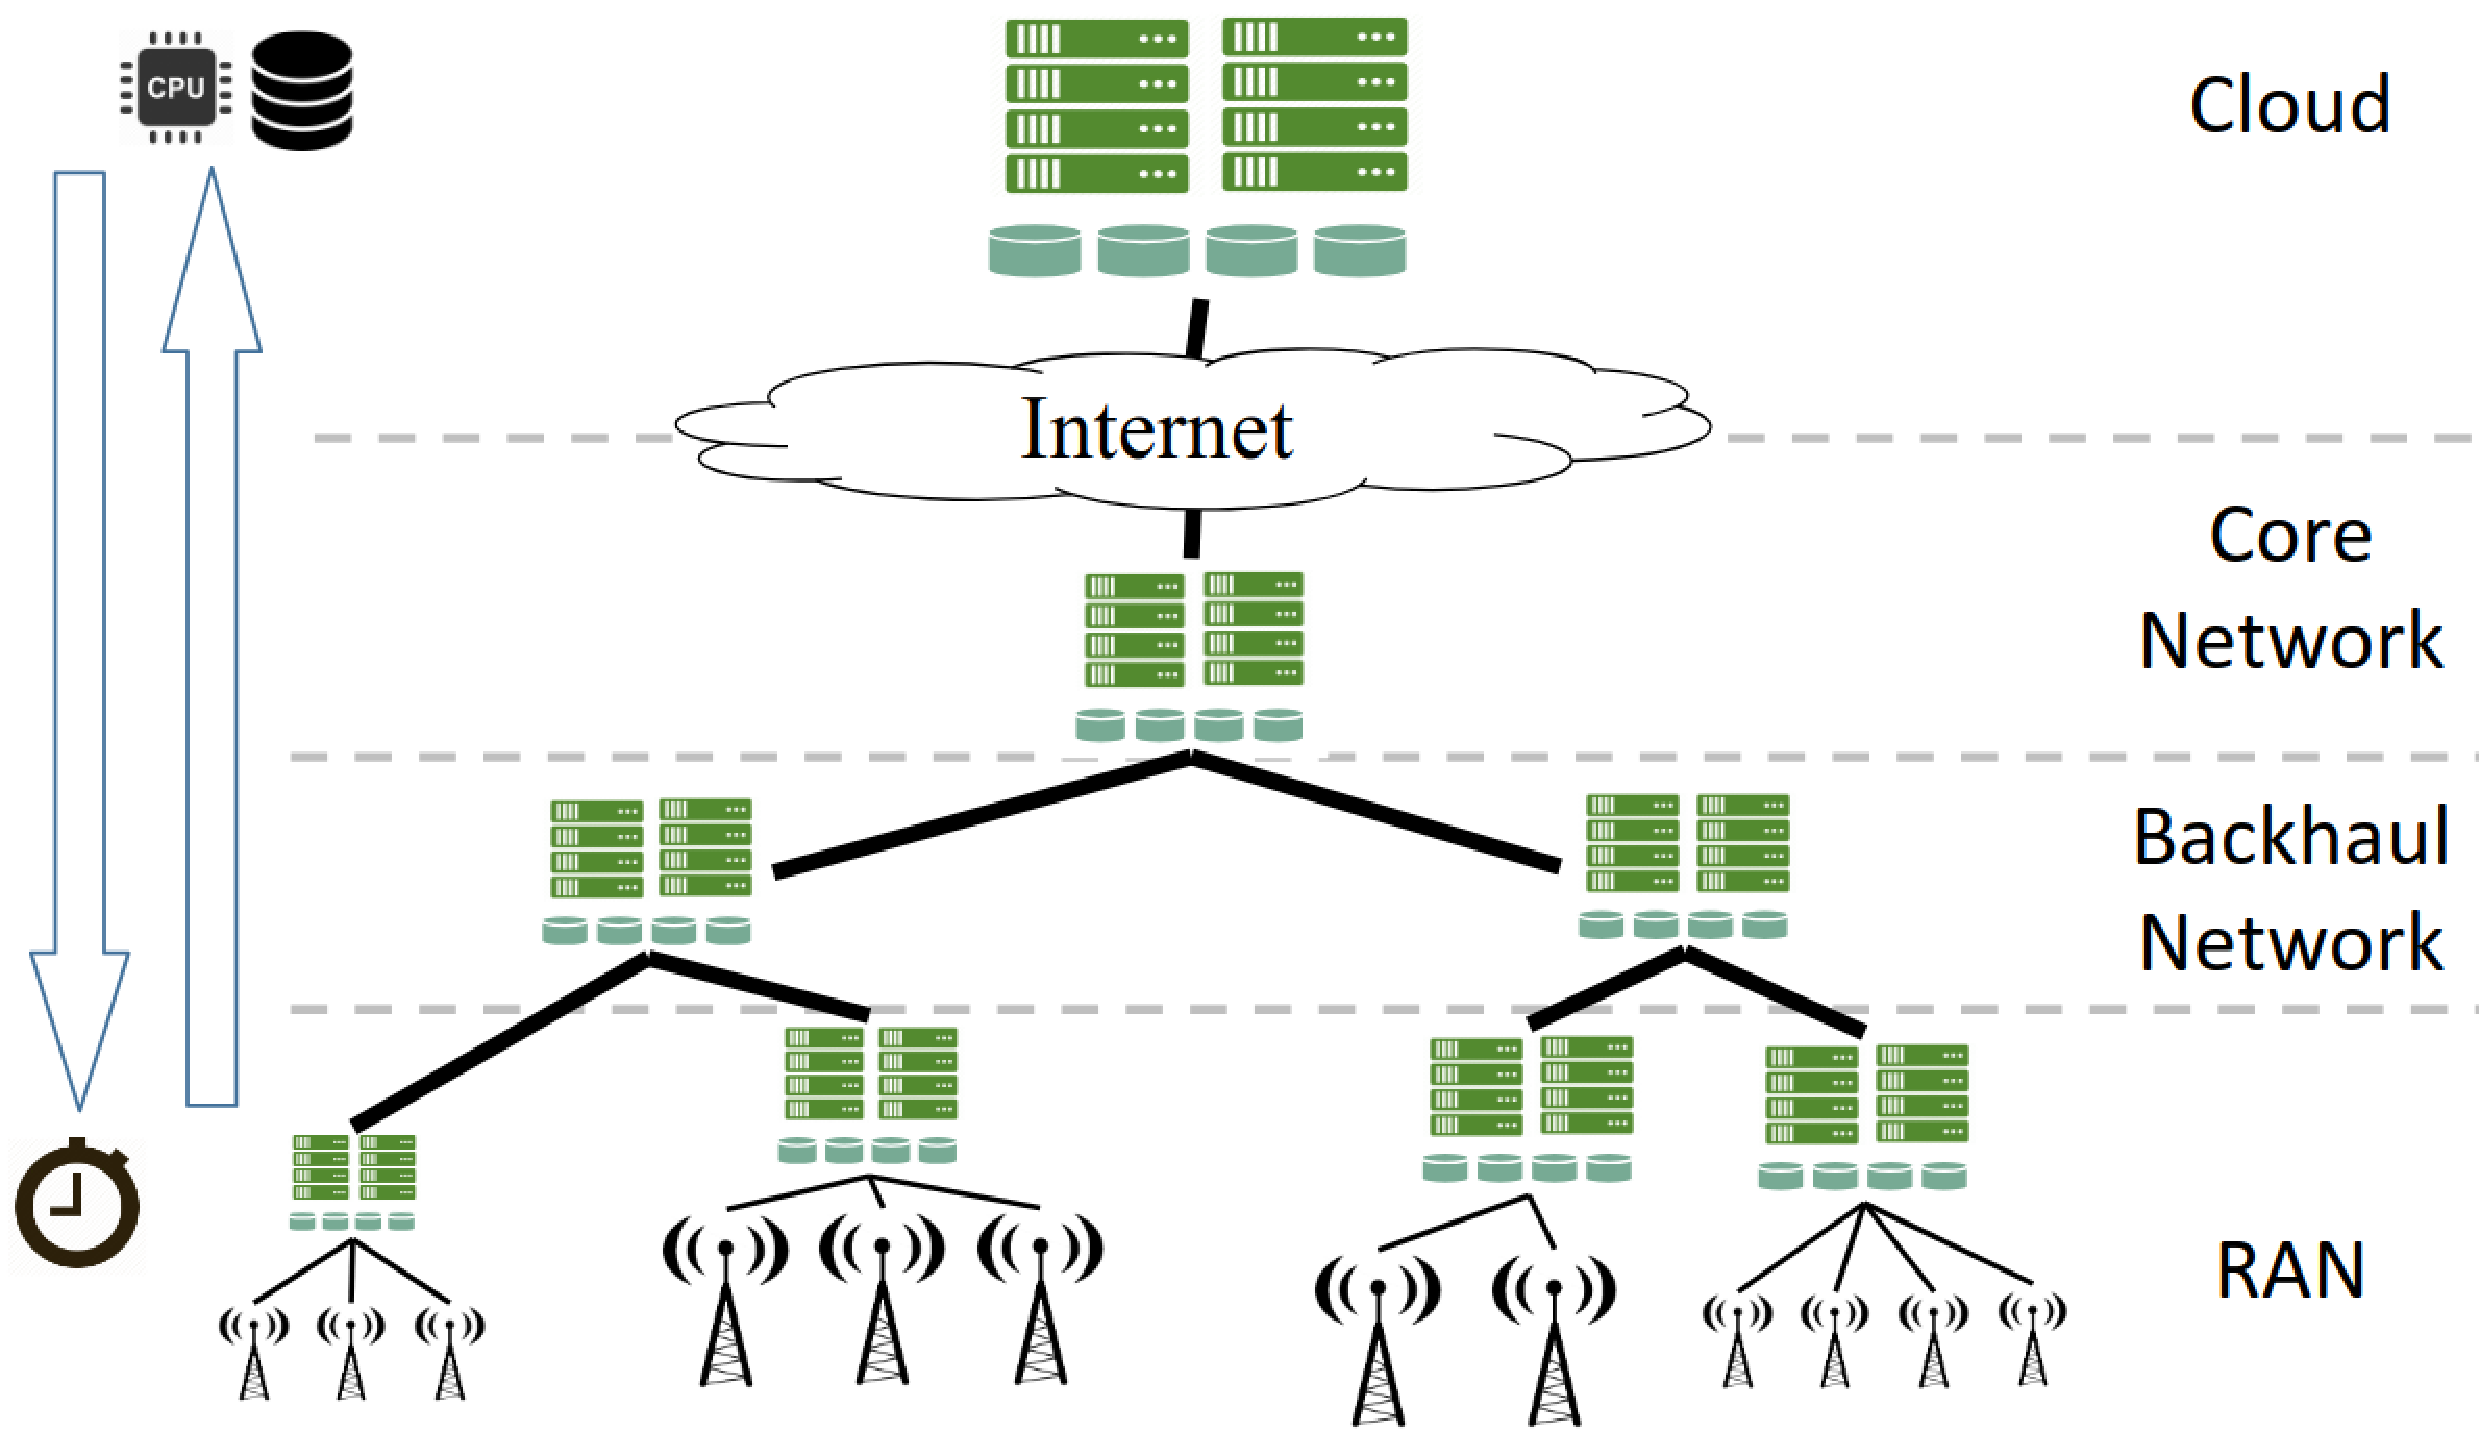
\includegraphics[width=0.9\linewidth]{img/5g/mec}
\end{center}

Si vogliono avere risorse a ogni livello (Cloud Edge Continuum), ovviamente con limitazioni su applicazioni contenute e capacità disponibile.

Le domande sono: 
\begin{itemize}
	\item Dove installare i vari moduli? Cloud? MEC server? Dispositivo stesso? 
	
    \item Come viene gestita la mobilità dei dispositivi che utilizzano il servizio?
\end{itemize}

La risposta dipende dai requisiti del modulo e dei link di comunicazione tra moduli.

Vantaggi: 
\begin{itemize}
	\item Architettura fortemente decentralizzata e localizzata

	\item Riduzione della latenza e jitter end-to-end

	\item Riduzione traffico verso il core della network

	\item Migliore supporto a Servizi Location/Context-Aware
\end{itemize}

Sfide: 
\begin{itemize}
	\item Integrazione nella rete: Come coesistono MEC e standard 3GPP? Come viene garantita la trasparenza a UE?
    
	\item Portabilità delle applicazioni MEC, Allocazione e de-allocazione trasparenti e impercettibili (seamless); Architetture HW e SW standard e open

	\item Sicurezza; Come viene garantito l'isolamento tra le VM nei MEC server? Come controllare dinamicamente l'uso corretto delle risorse dell'operatore?

	\item Performance; Dimensionamento delle VM; Allocazione ottimizzata delle VM all'interno della rete

	\item Resilienza
\end{itemize}

\subsection{Network Slicing}

Network slicing è un concetto che trasforma la rete/sistema  da \textbf{paradigma} statico a uno \textbf{dinamico} (nei primi standard si avevano qualità di servizio predefinite, qualunque fosse il servizio), nel quale \textbf{reti logiche} vengono create \textbf{on demand} con risorse e topologie ottimizzate per servire uno scopo specifico, una categoria di servizi o singoli utenti.

\textbf{Network Slice Instance} è un insieme di network function e risorse di rete organizzate e configurate in modo da fornire una rete logica che soddisfa certe caratteristiche.

Per ogni classe di servizio/esigenza viene costruito un overlay di rete ad hoc, al di sopra della rete fisica. Diventa molto più flessibile la gestione della rete \textit{al servizio di un servizio}, viene creata una slice della rete ad hoc per il servizio specifico.

5G abbandona l'idea degli standard precedenti in cui \textit{one size fits all}, esistono diversi casi d'uso e le risorse vengono allocate di conseguenza.

%End L20

\subsection{Architettura}

\subsubsection{LTE CUPS (Control User Plane Separation)}

Un po' di "storia": due release prima di 5G effettivo (Rel-14, 5G è la 16, quindi si parla ancora di LTE, anche se 6 release dopo la prima release LTE). 
\begin{center}
	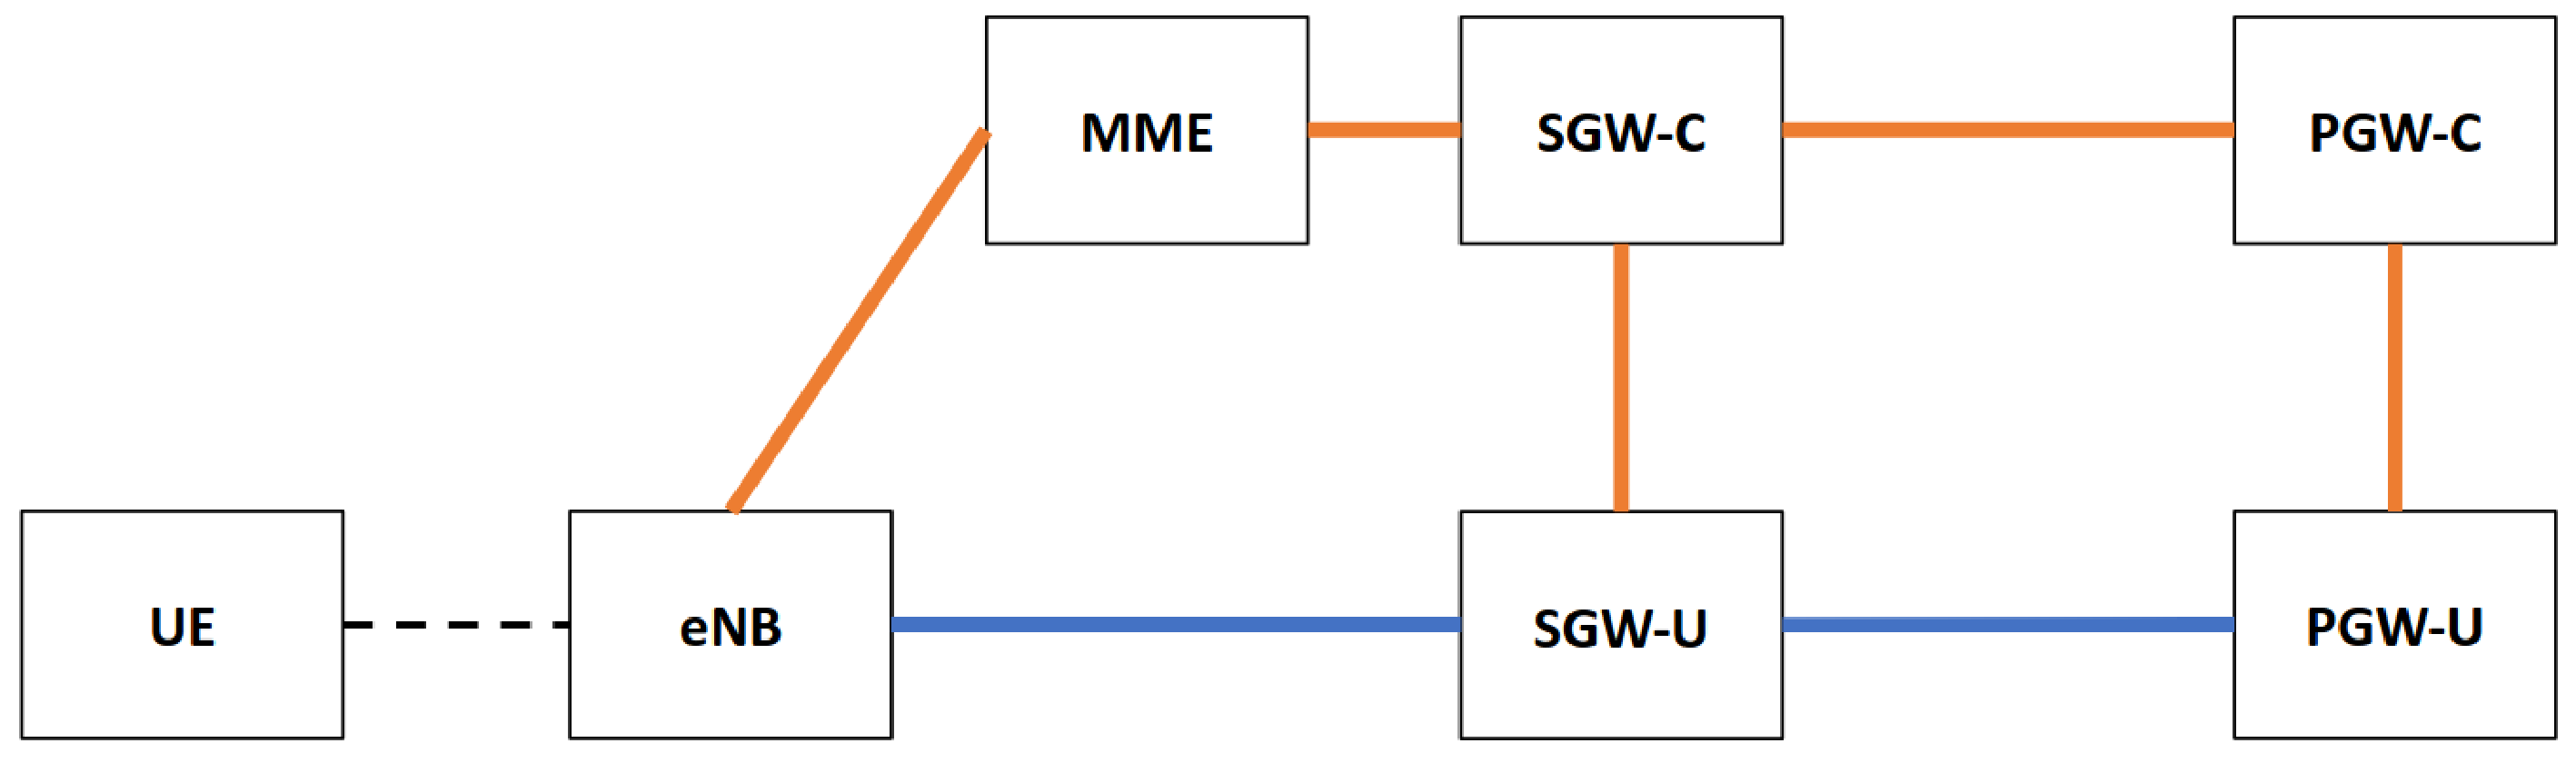
\includegraphics[width=0.9\linewidth]{img/5g/ltecups}
\end{center}

Si ha una \textbf{separazione} tra \textbf{user plane e control plane} in modo che siano indipendenti l'uno dall'altro, permettendo una migliore scalabilità, indipendente tra i due piani (ognuno dei due può essere scalato senza che l'altro vada necessariamente modificato). 

\subsubsection{Divisione dei Plane}

In 5G, rispetto le versioni precedenti, si ha un \textbf{data plane semplificato} quasi all'estremo (un solo componente che si occupa del controllo), mentre il \textbf{control plane prevede} una sempre \textbf{\textbf{maggior divisione dei compiti}} su componenti diverse.
\begin{center}
	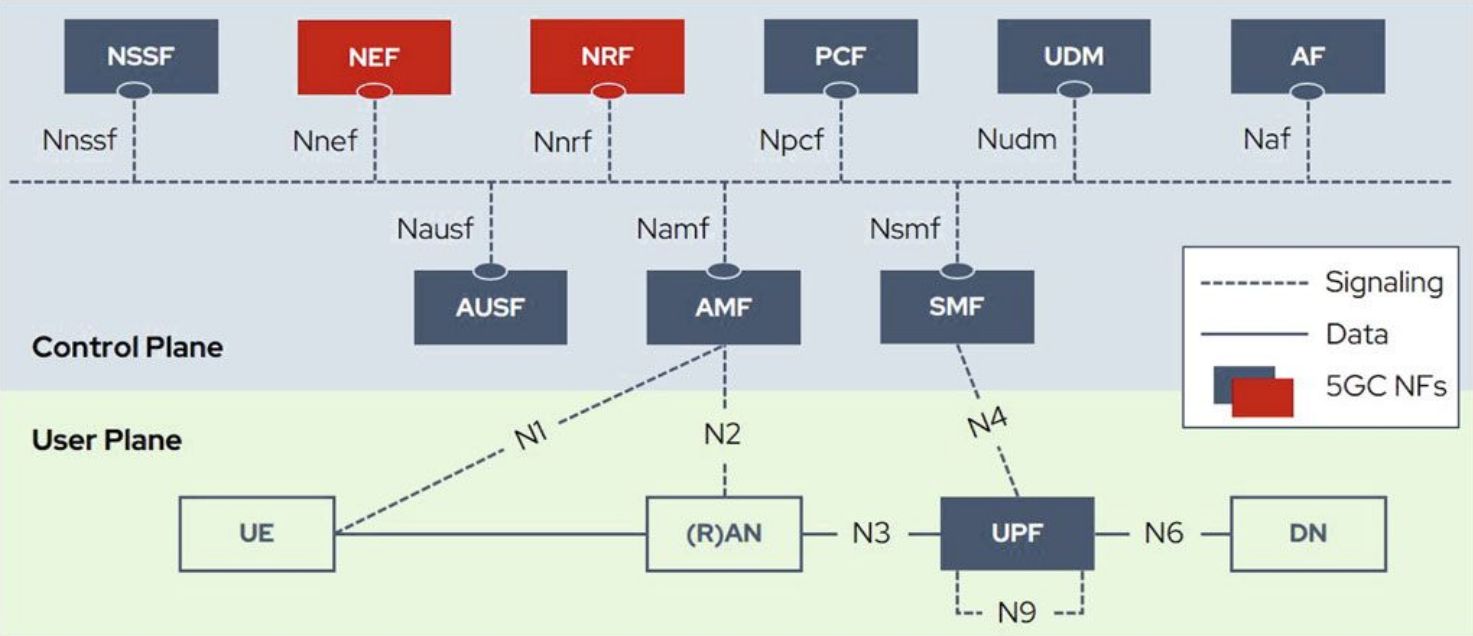
\includegraphics[width=0.98\linewidth]{img/5g/arch}
\end{center}

La parte di comunicazione all'interno di data plane e tra i due piani rimane strutturata come una comunicazione punto-punto tra i vari componenti. 

All'interno del control plane viene usata una \textbf{service-based architecture} con un \textbf{modello publish-subscribe}: ogni componente è una VNF e ognuna di queste implementa un servizio con API REST. Ogni VNF può consumare una o più API delle altre VNF. Si ha un bus comune di comunicazione tra tutte le VNF.

Ogni componente del control plane è una VFN, quindi ognuno può evolvere indipendentemente, ogni VNF può essere (dis)attivata o scalata in base alla necessità. Sono presenti tanti "micro-servizi" che svolgono le funzioni precedentemente svolte dal control plane.

\paragraph{Control Plane:} All'interno del control plane si trovano
\begin{itemize}
	\item \textbf{NRF Network Repository Function}: permette a ogni servizio di registrarsi e rendersi individuabile dalle altre VNF
	
	\item \textbf{AMF Access \& Mobility Management Function}: gestisce la maggior parte del traffico di segnalazione per autenticazione, registrazione e mobilità; una delle 3 parti in cui è stato diviso quello che era l'MME, gestisce una parte delle funzionalità precedentemente svolte dall'MME ma non gestisce dati di sessione (compito dell'SMF)
	
	\item \textbf{SMF Session Management Function}: Gestisce il controllo relativo alla creazione di sessioni dati; permette di creare delle sessioni user plane; unico componente che comunica con l'unica funzionalità core del data plane (ovvero la User Plane Function UPF)
	
	\item \textbf{UDM Unified Data Management Function}: fornisce un front-end unico per tutti i dati che ciascuna funzionalità di rete può richiedere; ogni NF può aver bisogno di dati diversi (strutturati, non-strutturati, semi-strutturati); qualsiasi NF che richiede un qualche tipo di database effettua le richieste di dati qua
	
	\item \textbf{PCF Policy Control Function}: effettua la parte di gestione e controllo delle politiche di accesso/mobilità in rete e di utilizzo dello user plane (prima dato alle PCRF)
	
	\item \textbf{AUSF Authentication Server Function}: gestisce tutto ciò che riguarda l'autenticazione e la generazione delle chiavi di cifratura
	
	\item \textbf{NSSF Network Slice Selection Function}: la funzione che dice quale può essere la slice migliore e consentita per un determinato servizio richiesto da un determinato utente
	
	\item \textbf{NEF Network Exposure Function e AF Application Function}: per integrare e permettere di utilizzare più informazioni; la NEF espone all'esterno della rete delle funzionalità, la AF permette all'applicazione di rendersi visibile all'interno della rete core; permettono alla rete e alle applicazioni/servizi esterni di dialogare tra loro esponendo funzionalità
\end{itemize}

\paragraph{User Plane:} Semplificato, rispetto alle release precedenti: 
\begin{itemize}
	\item \textbf{UE User Equipment}

	\item \textbf{RAN}: composta da gNodeB (per distinguerla dalle precedenti principalmente), gestisce la parte radio (link allo UE)

	\item \textbf{UPF User Plane Function}: unica componente dello user plane, si occupa dell'inoltro dei pacchetti utente da/verso l'esterno (DN); il loop con interfaccia N9 permette routing tra data network

	\item \textbf{DN Data Network}: rete esterna
\end{itemize}

\paragraph{Protocol Data Unit PDU:} I pacchetti utente viaggiano all'interno di una connessione end-to-end sullo user plane chiamata PDU session. 

La sessione va da uno UE a uno specifico DN, si tratta di una connessione dal device alla rete esterna (DN). Al di sopra si ha il livello applicativo, al di sotto uno stack (idealmente) IP-MAC-PHY.

Lo stack di protocolli lato user plane rimane simile a quello 4G (con le necessarie modifiche per la PDU).

\paragraph{Multiple PDU Sessions:} Un singolo UE può avere più connessioni attive, verso diverse data network, attraverso diverse UPF. Viene utilizzata una UPF per ogni collegamento.

\paragraph{Interfaccia N9:} Permette di connettere tra loro più UPF e fare routing verso altre data network. Per fare ciò si usa un ulteriore UPF che classifica il traffico in downlink: chiamata \textbf{ULCL (UpLink CLassifier)}, questa viene configurata apposta per classificare il traffico in uplink di ciascun dispositivo, permettendo di fare routing verso la corretta Data Network in modo trasparente all'utente.

\subsubsection{Network Slices}

Si espandono le funzionalità dei TTF in 4G, i quali permettevano solo la configurazione di alcuni parametri di rete. 

Le \textbf{Network Slices 5G} permettono di \textbf{classificare diversi casi d'uso} e per ciascuno si hanno anche diversi siti di installazione delle diverse NF (a livello di distanza rispetto all'utente)
\begin{center}
	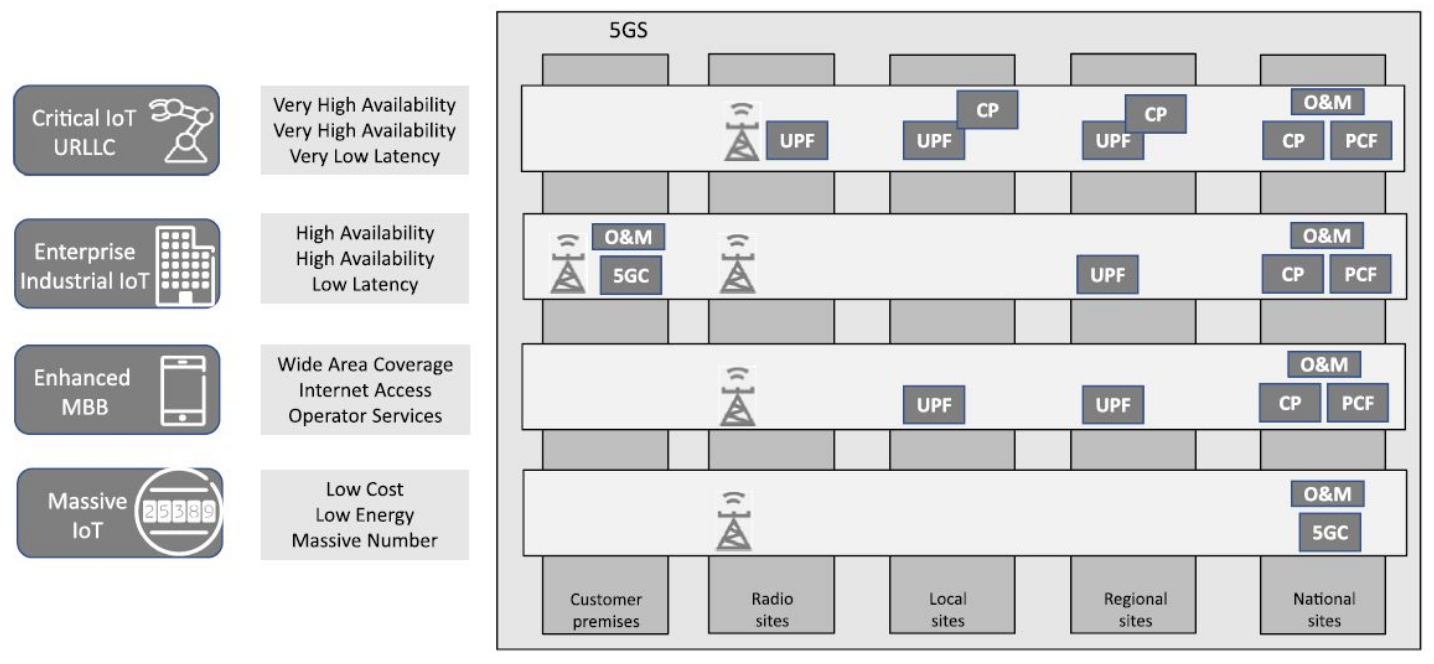
\includegraphics[width=0.99\linewidth]{img/5g/slicing}
\end{center}

Permette non solo di stabilire le \textbf{caratteristiche del servizio}, ma specifica anche la \textbf{composizione delle NF che permettono il servizio}. 

Rende possibile avere anche più livelli di Control Plane CP, per diversi servizi all'interno dello stesso caso d'uso (un servizio magari necessita di tempi di risposta molto brevi, ma gli altri no); l'uscita dalla rete può essere prevista in diversi punti, sempre in base al servizio (vedi Critical IoT URLLC). I servizi sono "confezionati" anche a livello di collegamenti logici tra NF.

Fornisce grande flessibilità alla rete oltre che alla qualità di servizio, tutto questo grazie alle tecnologie di virtualizzazione.

\paragraph{Identificazione:} Per l'identificazione della slice si usa uno slice identifier a 32 bit
\begin{center}
	\begin{tabular}{| C{2cm} | C{6cm} :}
		\multicolumn{2}{c}{Single-Network Slice Selection Assistance Information (S-NSSAI)} \\
		\cline{1-1} \cdashline{2-2}
		Slice Service Type (SST) \newline 8 bits & Slice Differentiator (SD) 24 bits \\
		\cline{1-1} \cdashline{2-2}
	\end{tabular}
\end{center}

I primi 8 bit indicano l'utilizzo per cui è pensata la network slice: 
\begin{center}
	\renewcommand{\arraystretch}{1.6}
	\begin{tabular}{| C{1.3cm} | C{1.2cm} | C{8.5cm} |}
		\hline
		0  & & Reserved \\
		\hline
		1  & eMBB & suitable for handling of 5G Enhanced Mobile Broadband \\
		\hline
		2  & URLLC & suitable for handling of Ultra-Reliable Low Latency Communications \\
		\hline
		3  & MIoT & suitable for handling of Massive IoT \\
		\hline
		4  & V2X & suitable for handling of V2X services \\
		\hline
		5-127  & & Reserved \\
		\hline
		128-255  & & Operator-specific \\
		\hline
	\end{tabular}
\end{center}

Mentre gli ultimi 24 definiscono la specifica istanza di un determinato tipo. 

La slice consentita all'utente viene determinata con il dialogo tra UE + AMF + NSSF + UDM. 

In questo modo il dispositivo è a conoscenza della slice a cui è assegnato e inserirà l'identificativo della slice all'interno dei pacchetti.

\subsubsection{5G e MEC}

L'integrazione tra 5G e MEC avviene tramite UPF come data plane nell'architettura MEC. 

UE che usa un servizio MEC ha UPF (PSA) collegato alla MEC platform dove è attivo il servizio che utilizza.

\subsubsection{5G RAN - 5G NR (New Radio)}

Vogliamo mantenere i 14 simboli OFDMA ma lo slot da $10ms$ non va bene, si vuole ridurre la latenza. 

La soluzione è \textbf{ridurre la durata dei simboli} (stesso numero, meno tempo), risparmiando banda.

Lo standard 5G NR definisce 5 diverse durate, indicate come \textbf{numerology}. Definisce anche due possibili intervalli di frequenze:
\begin{itemize}
	\item \textbf{FR1 (Frequency Range 1)}: 410MHz - 7125MHz

	\item \textbf{FR2 (Frequency Range 2)}: 24250MHz - 52600MHz
\end{itemize}

Di conseguenza, per una numerology $\mu$ si ha una $\Delta f$ (distanza tra le frequenze) calcolabile come
$$ \Delta f = 2^\mu \cdot 15 [kHz] $$
\begin{center}
    \renewcommand{\arraystretch}{1.5}
	\begin{tabular}{| C{1.5cm} | C{2cm} | C{3cm} | C{2cm} | C{2cm} |}
		\hline
		$\mu$ & $\Delta f$ & Cyclic Prefix & Banda di frequenza & Utilizzo  \\
		\hline
		0 & 15 & Normal & FR1 & Dati \\
		\cline{1-4}
		1 & 30 & Normal & FR1 & e \\
		\cline{1-4}
		2 & 60 & Normal, Extended & FR1 \& FR2 & Controllo \\
		\cline{1-4}
		3 & 120 & Normal & FR2 & \\
		\hline
		4 & 240 & Normal & FR2 & Controllo \\
		\hline
	\end{tabular}
\end{center}

Quando aumenta la distanza tra le portanti si usa solo il secondo range di frequenze, considerevolmente più ampio, altrimenti non ci starebbero abbastanza utenti all'interno. 

Per formare un Resource Block con 21 subcarrier serve, in base alla numerology, un range di
\begin{center}
	\begin{tabular}{ c | c | c | c | c | c}
		$\mu$ & 0 & 1 & 2 & 3 & 4 \\
		\hline
		& 180kHz & 360kHz & 720kHz & 1,44MHz & 2,88MHz 
	\end{tabular}
\end{center}

Raddoppiare la banda permette di dimezzare il tempo necessario per ogni simbolo. 

All'interno dello scheduling si possono allocare resource block con numerology diverse, magari anche in base alla slice utilizzata. 

Oltre alla rete, anche la configurazione della radio si può adattare all'utilizzo (se richiede latenza bassa si aumenterà la banda e diminuirà la durata del simbolo).

%End L22